This chapter study the syntactic transformation of \oz{} class into \picalc{} process. The resulting processes is intuitively defined as follow:\\
$P_{OZ\_part\_as\_\pi\_process} = \sqcap _{v\_st}\ Q(v\_st,v\_self)$\\
$Q(v\_st,v\_self) = (\Box _{c,v\_in_{c}} \sqcap _{v\_st'} \ c.v\_in_{c} \ + \ \Box _{c,v\_out_{c}} \sqcap _{v\_st'} \ c.v\_out_{c})\rightarrow \ Q(v\_st',v\_self)$
where:
\begin{itemize}
\item $c$ refers to an operation.
\item $v\_st$ refers to the state variables.
\item $v\_self$ refers to the instance reference.
\item $c.v\_in_{c}$ refers to the occurrence of the operation $c$, where $v\_in_{c}$ represents the values of the input parameters of $c$.
\item $c.v\_out_{c}$ refers to the occurrence of the operation $c$, where $v\_out_{c}$ represents the values of the output parameters of $c$.
\item $\Box$ deterministic choice, $\sqcap$ non deterministic choice, $+$ choice.
\end{itemize}
\textbf{Question 1:} what is the benefit of transformating an \oz{} class into \picalc{} process?\\
\textbf{Answer:} to combine it, using parallel operator, with a second \picalc{} processes.
\textbf{Question 2:} what is the benefit of the  second processes?\\
\textbf{Answer:} the second processes represents sequences of behavior. This will enable us to study the behavior of an entity as will be shown later in the next chapter.

To transform \oz{} class into \picalc{} process we need to remember that  \picalc{} has only names and processes, and nothing other. Thus, need to names and processes to represent: value, state variable, state schema, initial state schema and operation schema in \picalc{}. The rest of this chapter 
\section{Mapping values}
\label{sec_tra_oz_mapping_values}
In this thesis we restrict ourselves to two bits binary numbers shown \refTab{two_bit_binary_numbers}. A value can be mapped to a \picalc{} processes. \refLis{values_ABC_code} shows the \picalc{} implantation of the values 0,1,2,3 in ABC syntax. The keyword \textbf{agent} defines a new processes. The process $Zero$ receives two channels $tt,ff$ via the channel $a$, then it sends two signals via the channel $ff$. A value will be deleted when it receives a signal via $a$.
\begin{table}[H]
\centering
\begin{tabular}{|c|c|}
\hline
Decimal & Binary \\ \hline
0       & 00     \\ \hline
1       & 01     \\ \hline
2       & 10     \\ \hline
3       & 11     \\ \hline
\end{tabular}%
\caption{Two bits binary numbers.}
\label{two_bit_binary_numbers}
\end{table}
\lstinputlisting[backgroundcolor=\color{white},caption={0,1,2,3 as \picalc{} processes.},captionpos=b, label={values_ABC_code}]{listings/values.abc}


\section{Mapping Data Types}
\label{sec_tra_oz_mapping_data_types}
For simplicity, we do not implement any kind of type checking, but we deal with types by representing the value of the type by corresponding process. For example $cv: \{0,1,2,3\}$, means that the allowed processes to be initialized with $cv$ are: $Zero, One, Two, Three$.

\section{Mapping state variables}
\label{sec_tra_oz_mapping_state_variables}
A variable can be mapped to a channel. Creating a variable $x$ and initializing it with the value $0$ ( int x = 0;) is mapped to creating a new channel x and initialize the processes Zero with the channel x
as shown in \refFig{fig_oz_unfixed_operation_schema_shop}. The wide hat refers to creating a new channel.
\begin{figure}[H]%
\centering
\subcaptionbox{Abc code.}{\fbox{$(\ \widehat{}\ \text{x}\ )\ (\ \text{Zero}(\text{x})\ )$}}%
\hspace{1em}%
\subcaptionbox{visualization.}{\fbox{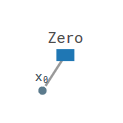
\includegraphics[]{./images/transformational_semantics_of_oz/var.png}}}%
\caption{variable as a channel}
\label{tra_var}%
\end{figure}


\section{Mapping class}
\label{sec_tra_oz_mapping_class}
\begin{figure}
\begin{subfigure}{.5\textwidth}
  \centering
\begin{class}{IdleShop(id: \integer)}
\begin{state}
m, vmId, self: \integer
\\t: nil | talk
\end{state} 
\\
\begin{init}
\\self = id
\\t = nil
\end{init} 
\\
\begin{op}{switch\_\_\_\_\ then\ ActiveShop}
\Delta (t)
\\x?: nil | talk
\ST
x? = t'
\end{op}
\end{class}
  \caption{1a}
  \label{fig:sfig1}
\end{subfigure}%
\begin{subfigure}{.5\textwidth}
  \centering
\fbox{  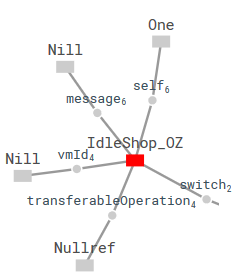
\includegraphics[width=.8\linewidth]{./images/transformational_semantics_of_oz/idleShop_OZ.png}}
  \caption{1b}
  \label{fig:sfig2}
\end{subfigure}
\vspace{2em}

\begin{subfigure}{1\textwidth}
  \centering
\lstinputlisting[backgroundcolor=\color{white},caption={ABC code: IdleShop OZ as a processes.},captionpos=b, label={idleShop_OZ}]{listings/idleShop_OZ.abc}
  \caption{1b}
  \label{fig:sfig3}
\end{subfigure}
\caption{transforming IdleShop}
\label{fig:fig}
\end{figure}

\section{Mapping state schema}
\label{sec_tra_oz_mapping_state_schema}
mapping

\section{Mapping initial state schema}
\label{sec_tra_oz_mapping_initial_state_schema}
mapping

\section{Mapping operation schema}
\label{sec_tra_oz_mapping_operation_schema}
mapping